\section{Local exploration and the transfer row}\label{c2:boundary}

We first determine the critical mass of a half-plane arch reaching height
$T$, and the corresponding strip and endpoint masses.  The exponent will
be $1/4$.  The calculation has two inputs: a positive bound from finite
boundary exploration, and an exact equation for arcs on a half-cylinder.
The latter requires a transfer row whose normalized fixed vector really
counts the physical arcs.  We construct that vector here and derive its
endpoint exchange equations; Section~\ref{sec:orbit} will solve them.

All positive path sums use the critical vertex weight
$x=(2\cos(\pi/8))^{-1}$ from the introduction.  A path specified by an
unordered pair of endpoints is counted once.  We use $\lesssim$ for an
upper bound up to a scale-independent constant, and $\asymp$ for bounds
in both directions.

\subsection{Finite exploration and a positive arch bound}

Write $\mathbf a_{jk}=jU+kV$ and $\mathbf b_{jk}=\mathbf a_{jk}+e_0$.
Use the half-plane consisting of the vertices with $k\ge0$, above the
bottom wall $e_2\cdot z=1/2$.  Let $h(d)$ be the mass of finite paths from
$e_2/2$ to $e_2/2+dU$, for $d\in\mathbb Z\setminus\{0\}$.  A multipath
is a collection of paths with disjoint vertices and distinct endpoints.

Put
\[
 s=3/8,\qquad \lambda=\pi/8,\qquad r=\pi s,\qquad c=2\cos r.
\]
The following finite exploration is a nonbacktracking form of the
honeycomb parafermionic cancellation~\cite{DuminilCopinSmirnov2012}.
Let $D$ be a bounded convex polygon cut out by the admissible lines
$e_\nu\cdot z\in1/2+(3/2)\mathbb Z$.  These lines avoid lattice
vertices and cut edges orthogonally at their midpoints.  Indeed the
$e_\nu$-levels of the $\mathbf a$ vertices lie in $(3/2)\mathbb Z$,
and increments toward the $\mathbf b$ vertices are $1,-1/2,-1/2$.
Only one cut family passes through any port, so no port is a corner.

Start at a port $a$ and explore inward.  At each fresh vertex take the two
nonbacktracking turns by $\pm\pi/3$, with complex weights
$xe^{\pm\mathrm i s\pi/3}$.  Their sum is one.  Stop at the first exit
or the first repeated vertex, before choosing another turn there.  Thus a
fresh vertex contributes one factor $x$, while the terminal repeated
vertex contributes no new factor.  There are finitely many histories,
and their total complex weight is one.

A repeated-vertex history has a simple stem followed by one traversal
of a simple polygon.  The stem lies outside that polygon: it begins at
the exterior source and cannot cross the polygon before the first
repeat.  At their attachment the unused third honeycomb edge is therefore
exterior.  A counterclockwise traversal of the closed polygon has turn
$+\pi/3$ at the attachment; entering from the stem and departing around
the polygon replaces this by $-\pi/3$.  The two possible traversals
consequently add turns $+4\pi/3$ and $-4\pi/3$ relative to the incoming
stem.  Their phase ratio is $e^{\mathrm i s(8\pi/3)}=-1$, so all
repeat histories cancel in pairs.

For a simple exit path from $a$ to $b$, its turn $W_{ab}$ depends only on
the ports.  It is the lifted increase of the outward-normal angle along
the counterclockwise boundary from $a$ to $b$, minus $\pi$.  To see this,
close the chord by the complementary counterclockwise boundary arc.
The resulting Jordan polygon has total turn $2\pi$ and contributes
$+\pi/2$ at each of the two joins.  In particular $|W_{ab}|\le\pi$.
Writing $h_D(a,b)$ for the positive mass of chords in $D$, we obtain
\begin{equation}
 \sum_b e^{\mathrm i sW_{ab}}h_D(a,b)=1.
 \label{c2:eq-1}
\end{equation}
Every summand's real part is at least its positive mass times
$\cos(\pi s)>0$.  Exhaust the half-plane by adding cuts
$e_\nu\cdot z\le M$, $\nu=0,1$, on the admissible grids.  Bottom
exits to the right and left have turns $-\pi$ and $+\pi$, respectively.
Monotone convergence of their positive masses and reflection symmetry give
\begin{equation}
 h(d)=h(-d),\qquad c\sum_{d>0}h(d)\le1.
 \label{c2:eq-2}
\end{equation}
This bound will control every component of the finite-cylinder transfer
vector without assuming the boundary exponent that we seek.

\subsection{The local diagram weights and braid identity}

We use the trigonometric dilute-loop weights in
\cite{GlazmanManolescu2017}.  The normalized coefficients below also
follow by dividing the weights in \cite[Eq.~(1.2)]{ZhouBatchelor1997}
by their empty-tile weight.  Their diagram algebra is the braid--monoid
calculus of Grimm and Pearce~\cite[Eq.~(4.20)]{GrimmPearce1993}.
Boundary contractions depend on the gauge.  We therefore fix the
coefficients explicitly and verify the braid identity in this
normalization.  This identity will let an adjacent column exchange pass
through the transfer row.

Put \(S=3\lambda,\ a_0=2\lambda,\ b=\sin(2\lambda)=\cos(2\lambda),\ d=\sin(3\lambda)=\cos\lambda\), and
\[
 P_u=\sin u,\quad Q_u=\sin(S-u),\quad I_u=\sin(a_0-u),\quad J_u=\sin(u-\lambda).
\]
Make a two-strand braid box \(\check R(u)\) with ports in order input left, input right, output right, output left around the box. Use weights below, all divided by \(T_u\):
\[
\begin{array}{c|c}
\text{configuration}&\text{numerator}\\ \hline
\emptyset &T_u=bd+P_uQ_u=\sin(2\lambda+u)\sin(3\lambda+u)\\
\text{one strand at the same position in/out}& A_u=bQ_u\\
\text{one input cap or one output cup}& B_u=bP_u\\
\text{one strand changing position}& C_u=P_uQ_u\\
\text{both through at same positions}& D_u=I_u Q_u\\
\text{cap and cup}& E_u=J_u P_u .
\end{array}
\]
Figure~\ref{fig:box-order}(a) fixes the cyclic order used by the table.
A rotation of a box rotates its ports and connectivities together.

Only noncrossing diagrams are used. In compositions sum linearly over compatible diagrams (occupancies must match at glued ports, and strands concatenate), discarding terms with any closed loop. An untouched line has the vacant identity term and the single through-strand identity term.

In this calculus the boxes satisfy the additive braid identity
\begin{equation}
 \check R_1(v)\check R_2(u+v)\check R_1(u)=
 \check R_2(u)\check R_1(u+v)\check R_2(v),                              \label{c2:eq-3}
\end{equation}
where the subscripts are first and second neighboring pairs among three lines. Here is a verification using unnormalized weights (the denominators are common). Under \(u\mapsto S-u\) the box turns a quarter turn in the diagram sense, i.e. \(A,B\) exchange and \(D,E\) exchange (other weights unchanged). 

In the three boxes of the left side of \eqref{c2:eq-3} the six external ports in order (three inputs left to right, then three outputs right to left) belong in consecutive pairs to the first, middle and last crossings (input first ordering). The remaining ports form the internal triangle (each box connects to the next and the previous). Thus write the external pairs as \(L_i,R_i;\ L_j,R_j;\ L_k,R_k\) in cyclic order, with box parameters \(i,j,k\) respectively, satisfying \(i+j+k=S\) (these parameters are \(u,S-u-v,v\); the middle box has used the quarter turn). In each box \(B\) pairs the two exterior (or two interior) ports, and \(A\) connects an exterior port to the nearest interior port (\(R\) towards the next tile, \(L\) towards the previous); \(D\) gives both latter connections, \(E\) gives both caps, \(C\) gives one opposite connection. 

For the right side of \eqref{c2:eq-3} the whole placement, with the parameters, shifts by three external ports (the \(u\)-box is now last at outputs three and two, and the \(v\)-box first at inputs two and three). We just need invariance of all connectivity weights under this inversion of the boundary data.

Figure~\ref{fig:box-order}(b) records this triangle incidence and the
boundary inversion.  The picture allows the connectivity comparison to
be made independently of geometric rhombus angles.
\begin{figure}[htbp]
\centering
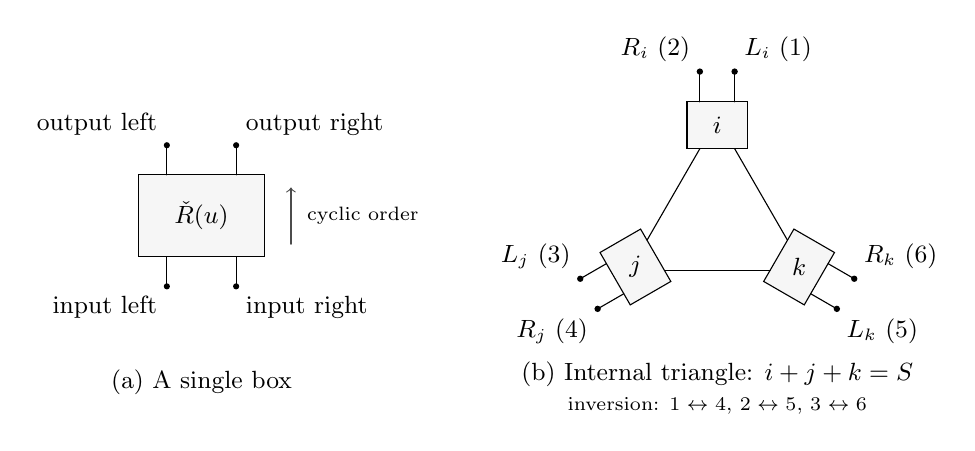
\begin{tikzpicture}[line cap=round,font=\small]
\begin{scope}[xshift=-3.35cm,yshift=.15cm,scale=.8]
\draw[fill=gray!7] (-1,-.65) rectangle (1,.65);
\node at (0,0) {$\check R(u)$};
\foreach \x in {-.55,.55}
  {\draw (\x,-1.12)--(\x,-.65); \draw (\x,.65)--(\x,1.12);}
\fill (-.55,-1.12) circle (1.4pt) node[below left] {input left};
\fill (.55,-1.12) circle (1.4pt) node[below right] {input right};
\fill (.55,1.12) circle (1.4pt) node[above right] {output right};
\fill (-.55,1.12) circle (1.4pt) node[above left] {output left};
\draw[->,black!70] (1.42,-.45)--(1.42,.45);
\node[anchor=west,font=\scriptsize] at (1.52,0) {cyclic order};
\node at (0,-2.65) {(a) A single box};
\end{scope}
\begin{scope}[xshift=3.2cm,yshift=.1cm,scale=.96]
\foreach \ang/\lab in {0/i,120/j,240/k}{
  \begin{scope}[rotate=\ang]
  \draw[fill=gray!7] (-.40,.94) rectangle (.40,1.56);
  \draw (-.23,1.56)--(-.23,1.96);
  \draw (.23,1.56)--(.23,1.96);
  \coordinate (\lab-next) at (-.23,.94);
  \coordinate (\lab-prev) at (.23,.94);
  \coordinate (\lab-L) at (.23,1.96);
  \coordinate (\lab-R) at (-.23,1.96);
  \end{scope}
}
\draw (i-next)--(j-prev);
\draw (j-next)--(k-prev);
\draw (k-next)--(i-prev);
\node at (90:1.25) {$i$};
\node at (210:1.25) {$j$};
\node at (330:1.25) {$k$};
\foreach \lab in {i,j,k}{
  \fill (\lab-L) circle (1.2pt);
  \fill (\lab-R) circle (1.2pt);
}
\node[above right] at (i-L) {$L_i\ (1)$};
\node[above left] at (i-R) {$R_i\ (2)$};
\node[above left] at (j-L) {$L_j\ (3)$};
\node[below left] at (j-R) {$R_j\ (4)$};
\node[below right] at (k-L) {$L_k\ (5)$};
\node[above right] at (k-R) {$R_k\ (6)$};
\node at (0,-2.05) {(b) Internal triangle: $i+j+k=S$};
\node[font=\scriptsize] at (0,-2.46)
  {inversion: $1\leftrightarrow4$, $2\leftrightarrow5$, $3\leftrightarrow6$};
\end{scope}
\end{tikzpicture}

\caption{(a) The four ports of a braid box, in cyclic order.
(b) After rotating the middle box in the three-box product, the exterior
ports occur in the numbered cyclic order shown.  An edge between boxes
is a glued internal edge.  The opposite product uses the boundary data
shifted by three positions, as indicated.  The picture records incidence
and cyclic order, rather than geometric rhombus angles.}
\label{fig:box-order}
\end{figure}

Here is the nontrivial scalar list for this comparison (up to cyclic triangle symmetry, reflection and reversing the comparison):
\[
\begin{array}{l|ll}
 &\text{weight}&\text{after inversion}\\\hline
 2\text{ ports}, L_i,R_i
     &B_iT_jT_k+D_iB_jB_k&T_i A_j A_k+B_i C_j C_k\\
 2,\ L_i,L_j
     &C_i A_j T_k+A_i C_j B_k&A_j C_k T_i+C_j A_k B_i\\
 4,\ L_i,R_i\text{ absent}
     &T_i B_jB_k+B_i(D_jE_k+E_jD_k)& D_i A_j A_k\\
     &B_i D_jD_k & B_i C_j C_k+E_i A_j A_k\\
 4,\ L_i,L_j\text{ absent}
     & A_i C_j B_k+C_i A_j E_k & A_j C_k D_i\\
 6   &B_iB_jB_k+\sum_{\rm cyc} D_i E_j E_k &D_iD_jD_k .
\end{array}
\]
For example, in the first line only $L_i,R_i$ are occupied.
They can pair directly in box $i$, leaving boxes $j,k$ empty, with weight
$B_iT_jT_k$.  Otherwise $D_i$ sends both endpoints into the triangle,
and caps in $j,k$ complete the route, with weight $D_iB_jB_k$.
After inversion the active endpoints are $R_j,L_k$.  Their route through
the $j$--$k$ edge has weight $T_iA_jA_k$; the route through box $i$
has weight $B_iC_jC_k$.

Indeed internal occupancies have even parity combined with external ones at each box. For all exterior counts even per box, this means no internal strands or else all three internal edges active (a closed internal triangle contributes zero); for two odd counts they are linked by either of the two paths in the triangle, with the two possible pairings at any box having degree four. 

For four ports with \(L_i,R_i\) absent the first line for that case pairs the exterior pairs within \(j,k\), the second exchanges. With \(L_i,L_j\) absent the displayed line pairs \(R_i,R_j\) to each other and \(L_k,R_k\) to each other; the other equality just switches \(k,i\). The six-port comparison shown pairs within each exterior pair versus pairing across the gaps. Cases with only two opposite ports occupied or only two opposite absent have matchings themselves invariant under inversion, as do the three remaining matchings in the six-port case (those with one within-box exterior pair and one opposite pair). Together with the empty exterior this exhausts the cases: a two-site subset (occupied or absent) is at separation one, two or three along the hexagon.

For clarity the two columns agree by the following identities. \(Q_jQ_k=P_jP_k+dP_i\), \(C_j+C_k=C_i+2\cos i\,P_jP_k\), \(I_j I_k-P_jP_k=b J_i\), \(I_i Q_k-P_i J_k=b P_j\) by angle sums. The difference in line one, divided by \(b^2\), reduces to \(P_jP_k[D_i-bd+P_i\sin(S+i)]\), zero (\(D_i=T_{-i}\)). 

In line two use \(T=bd+C,\ C_i-C_k=P_j\sin(i-k)\), \(Q_iP_k-Q_kP_i=d\sin(k-i)\). In line four cancel \(bP_i Q_jQ_k\) to use \(I_jI_k=P_jP_k+bJ_i\), and in line five cancel \(b Q_i Q_j P_k\) to use \(I_iQ_k=bP_j+P_iJ_k\); as throughout one can check generic parameters and then continue. 

Line three, using \(Q_jQ_k=P_jP_k+dP_i\) and \(D_i-T_i=-2dP_i\cos i\), reduces to
\[
 D_j E_k+E_jD_k=bd(D_i-2\cos i\,P_jP_k).
\]
To check it put \(\tau_u=2u-\lambda\), so \(D_u=(d-\sin\tau_u)/2,\ E_u=(d-\cos\tau_u)/2\). The left hand side is \(d^2/2+\cos(2i)/4-bd\cos i\cos(j-k)\) using \(\tau_j+\tau_k=4\lambda-2i\); \(D_i+\cos i\cos(S-i)=bd+\sin\lambda\cos(2i)\) and \(bd\sin\lambda=1/4\). 

Finally \(2(D_u+\mathrm i E_u)=d(1+\mathrm i)-\mathrm i e^{\mathrm i\lambda-2\mathrm i u}\), hence
\[
 8\,\Re\prod_{u=i,j,k}(D_u+\mathrm i E_u)
 =-bd+b\sum_{u=i,j,k}\sin(S-2u)=8b^3 P_iP_jP_k .
\]
Here expansion gives constant real part \(-2d^3+d=-bd\); the linear real part is \(\Re[d(e^{2\mathrm i\lambda}-\mathrm i)\sum_u e^{-2\mathrm i u}]\) where \(d(e^{2\mathrm i\lambda}-\mathrm i)=b e^{-\mathrm i\lambda}\). Here also \(\sum_{u=i,j,k}\sin(S-2u)-\sin S=4P_iP_jP_k\). This checks line six (first for real parameters, so also analytically). This proves \eqref{c2:eq-3} as a meromorphic identity per disk connectivity, hence also when glued into larger diagrams.

\subsection{The physical half-cylinder vacuum}

The local identity now lets us compare neighboring rapidity orders.  Before
using it, we construct the analytic vector to which it will be applied
and identify its homogeneous coordinates with positive path masses.

Next take the quotient by \(N U\) (circle direction), \(N\ge3\), using the same half-plane bottom; closed loops of any kind will be given weight zero. Index the \(N\) cut ports \(1,\ldots,N\) cyclically in the positive \(U\) direction. A state at the cut records some ports paired by disjoint simple (compact) arcs in the upper half-cylinder, including for each pair the relative homotopy of that arc, equivalently which lifts of the ports are joined (modulo simultaneous translation by periods). Each arc, lifted, connects endpoints less than \(N\) spacings apart (otherwise endpoints interlace with those of a translate, impossible by disjointness in the half-plane; equality projecting to one endpoint is disallowed). The disk side of the arc at the cut thus gives an interval from one endpoint to the other in the positive circle direction (lifted left endpoint to lifted right endpoint). In particular there are finitely many states. Denote the mass of a single arc with interval from \(i\) to \(j\), \(i\ne j\), by \(H_{ij}(0)\); we will deform this to an analytic function \(H_{ij}(\boldsymbol\eta)\) near \(\boldsymbol\eta=0\).

Form a transfer row \(\mathcal T(\boldsymbol\eta)\) on cylinder states by sending an auxiliary line from left to right once around the circle across the \(N\) vertical lines (input above, output below), with \(\check R(\lambda+\eta_j)\) at the crossing with column \(j\). Thus a cell uses left, upper side as ordered input ports and lower, right side as ordered outputs. Glue the auxiliary ends, and as before discard any closed loops. At \(\eta_j=0\) all these cells describe exactly the weighted honeycomb trajectories: the cell with \(\mathbf a_{jk},\mathbf b_{jk}\) as its two vertices has its left and lower ports incident to the former (towards \(\mathbf b_{j-1,k},\mathbf b_{j,k-1}\)), and upper and right to the latter (towards \(\mathbf a_{j,k+1},\mathbf a_{j+1,k}\)). Thus successive cuts can be indexed by the same columns, with a translation in the actual plane between levels. At \(u=\lambda\) we have \(A_u/T_u=x,\ B_u/T_u=C_u/T_u=D_u/T_u=x^2,\ E_u=0\), precisely allowing the two vertices once each.

The empty component is preserved by a row: closing off any nonempty
input without an output would create a loop, whose weight is zero.
In a basis starting with the empty state the transfer matrix therefore has
block form
\[
 \begin{pmatrix}1&0\\ g&K\end{pmatrix}.
\]
At homogeneity, applying its $h$th power to the empty state gives
\[
 \mathcal T(0)^h\binom{1}{0}
 =\binom{1}{\sum_{m=0}^{h-1}K(0)^m g(0)}.
\]
These coordinates count multipaths in finite row stacks and are bounded
componentwise as $h$ increases.  For each prescribed state, lift its arcs
to the half-plane and discard mutual avoidance and avoidance of period
translates.  The resulting product of one-arc masses is finite by
\eqref{c2:eq-2}.

Every nonempty state is accessible with positive weight.  Its lifted cut
intervals form a periodic laminar family.  Remove an innermost pair whose
open interval contains no other active port, and construct the remaining
state inductively.  In one additional row below that stack, insert the
removed pair by a lower-to-right corner, horizontal passages along its
interval, and a left-to-lower corner at the other endpoint.  Propagate
all other active ports by single upper-to-lower strands in their columns.
All these homogeneous weights are positive, and the chosen open interval
has no active port to obstruct the insertion.

Write $e_\alpha$ for a coordinate vector of the nonempty-state space.
Accessibility gives an integer $j_\alpha\ge0$ and a constant
$C_\alpha<\infty$ such that
$e_\alpha\le C_\alpha K(0)^{j_\alpha}g(0)$ componentwise.  Hence
\[
 \sum_{m\ge0}K(0)^m e_\alpha
 \le C_\alpha\sum_{m\ge0}K(0)^{m+j_\alpha}g(0)<\infty.
\]
Thus $\sum_m K(0)^m$ converges entrywise.  In particular $1-K(0)$ is
invertible, and the normalized fixed vector
\[
 \Psi(\boldsymbol\eta)
 =\bigl(1,(1-K(\boldsymbol\eta))^{-1}g(\boldsymbol\eta)\bigr)
\]
exists analytically near zero and is unique with empty component one.
Positivity was used at homogeneity; the nearby coordinates may be complex.
Its single-arc components \(H_{ij}\) agree at homogeneity with the excursion sums above by increasing the finite row stacks from empty. It rotates covariantly by construction.

\paragraph{Endpoint exchange.}
For \(u=\eta_{\ell+1}-\eta_\ell\) and \(S_\ell\) the parameter swap (positions \(\ell,\ell+1\)), \eqref{c2:eq-3} moves the box \(\check R_\ell(u)\) through the row and intertwines it with the swapped row. Indeed the crossing parameters are differences of successive visiting lines' labels (right minus left for the ordered inputs, exchanging labels at outputs), with auxiliary label \(-\lambda\): at the two columns (take \(1\le\ell<N\)) formula \eqref{c2:eq-3} uses the ordered labels \(-\lambda,\eta_\ell,\eta_{\ell+1}\), sliding the column exchange from below the two auxiliary crossings to above them. Thus \(\check R_\ell(u)\Psi(\boldsymbol\eta)=\Psi(S_\ell\boldsymbol\eta)\) by uniqueness and preservation of the empty projection. The one-arc coordinates satisfy a closed system.  If one of \(i,j\) equals \(\ell\) or \(\ell+1\) and the other lies outside this pair, then
\[
 T_u H_{ij}(S_\ell\boldsymbol\eta)= A_u H_{ij}(\boldsymbol\eta)+ C_u H_{i'j'}(\boldsymbol\eta),
\]
where the prime switches \(\ell,\ell+1\) on indices. Moving one port across the neighbor preserves the oriented interval type.
For the two neighboring interval types the equations are
\begin{equation}
 \begin{split}
 T_u H_{\ell,\ell+1}(S_\ell\boldsymbol\eta)&=D_u H_{\ell,\ell+1}(\boldsymbol\eta)+B_u,\\
 T_u H_{\ell+1,\ell}(S_\ell\boldsymbol\eta)&=D_u H_{\ell+1,\ell}(\boldsymbol\eta).
 \end{split}                                                        \label{c2:eq-4}
\end{equation}
These equations use only one-arc coordinates.  Outside the exchanged pair,
occupancies are unchanged; inside it, a box cannot remove an additional
arc while retaining an active output port.  A cap on an already paired
input pair creates a loop and gives zero.  Insertion from the vacuum
creates only the short interval $\ell\to\ell+1$, explaining the source
term $B_u$.


\section{A rapidity orbit and an inverse-matrix formula}\label{sec:orbit}

The preceding construction gives analytic one-arc masses $H_{ij}$ near
homogeneity.  We now calculate a particular sum of these masses.  Put
$\gamma=2\lambda$, $q=e^{\mathrm i\gamma}$ and
$\kappa=q^{-1}-q$, so $q^2=\mathrm i$ and $q^3=-q^{-1}$.  For distinct
rapidities write $x_i=e^{2\mathrm i\eta_i}$; these multiplication
variables are separate from the critical path weight $x$.

\begin{proposition}[The half-cylinder inverse pairing]
\label{prop:boundary-inverse}
For $N\ge3$ and generic distinct rapidities sufficiently near zero, define
\[
 \mathcal C_{ij}=\frac1{x_i+q x_j}\qquad(1\le i,j\le N).
\]
Then
\begin{equation}
 \sum_i x_i-c\sum_{i\ne j}e^{\mathrm i(\eta_i+\eta_j)}
 H_{ij}(\boldsymbol\eta)
 ={\bf1}^{\mathsf T}(\mathcal C^{\mathsf T}+q\mathcal C)^{-1}{\bf1}.
 \label{c2:eq-9}
\end{equation}
The scalar pairing on the right has a removable continuation to a
neighborhood of homogeneous rapidities.  This does not assert that the
matrix inverse itself extends to coincident rapidities.
\end{proposition}

We prove the formula on a finite permutation orbit and then continue it.
The same Cauchy matrix will appear in the generalized eigenproblem
for the one-coordinate reduction.  Endpoint exchange first gives operators on the $N!$ points of that orbit.
An $N$-dimensional space of functions of one coordinate supplies their
spectral information.  We use that information to show that every operator
commuting with the endpoint transports is scalar, and finally compute the
scalar that sums the arc coordinates.

\subsection{Endpoint transport on a finite orbit}

Let \(N\) be fixed and work on the permutation orbit of \(\eta_j=(j-1)\epsilon\) for sufficiently small real \(\epsilon>0\). Functions live on \(N!\) tuples. The multiset of the $x_i$ is fixed throughout. Operators permuting variables in a function are \(s_l\) for the swap of \(l,l+1\) and \(\rho f(\eta)=f(\eta_2,\ldots,\eta_N,\eta_1)\). Put
\[
 \delta=\prod_{i<j}\sin(S+\eta_i-\eta_j),\quad \Omega=\delta\rho\delta^{-1},\qquad
 F_{ij}=\delta e^{\mathrm i(\eta_i+\eta_j-S)} H_{ij}.
\]
Thus \(\Omega\delta=\delta,\ \Omega F_{ij}=F_{i+1,j+1}\) using rotation covariance. Define, for \(l<N\) and \(u=\eta_{l+1}-\eta_l\),
\[
 g_l=\frac{\sin(\gamma+u)}{\sin u}\,s_l-\frac{b e^{\mathrm i u}}{\sin u}
 =A(x_l,x_{l+1})\,s_l+B(x_l,x_{l+1}),
 \quad B(v,w)=\kappa\,\frac w{w-v},\quad A=q^{-1}-B .
\]
By \eqref{c2:eq-4} and the single-endpoint equation preceding it,
applying $g_l$ to \(F_{ij}\) moves an endpoint at \(l\) to \(l+1\) if the other endpoint is not at \(l+1\) (leaving the order of the two labels fixed).
For the neighboring pair, with $g=g_1$, the two equations are
\begin{equation}
 (g+q)F_{12}=x_1(g-1)\delta,\qquad (g+q)F_{21}=0.                    \label{c2:eq-5}
\end{equation}
Indeed under the swap the \(\delta\) ratio (swapped over original) is \(\sin(S+u)/\sin(S-u)\). For a moving endpoint at \(l\), the swap also contributes \(e^{\mathrm i u}\) from its exponential, so the swapped term of \(g_l\) uses the multiplier \(e^{\mathrm i u}T_u/(P_u Q_u)\) relative to the original prefactor. The \(A_u\) term then cancels the unswapped multiplication of \(g_l\), and the \(C_u\) term gives the moved \(F\). With both sites occupied there is no extra swap exponential; \(I_u-be^{\mathrm i u}=-qP_u\), so only the source survives after adding \(q\). For the short neighboring arc equation it is
\(b e^{\mathrm i(\eta_1+\eta_2-S)}\delta/\sin(S-u)=x_1(g-1)\delta\), the latter by \(T_u-P_u Q_u=bd\), \(d-e^{\mathrm i u} Q_u=e^{\mathrm i(u-S)}P_u\).

We give details of the operator calculation on this orbit. The following relations hold:
\begin{equation}
 g_l^2=1+\kappa g_l,\quad g_l g_{l+1}g_l=g_{l+1}g_lg_{l+1},\quad
 [g_l,g_j]=0\ (|l-j|>1),\quad g_l x_l=x_{l+1}g_l^{-1},
                                                                    \label{c2:eq-6}
\end{equation}
for ordinary indices less than \(N\) (other \(x_j\) commute if \(j\ne l,l+1\)). These follow from the formulas: \(B(v,w)+B(w,v)=\kappa,\ A(v,w)A(w,v)=1+B(v,w)B(w,v)\), and on any triple \(v,w,z\)
\(B(v,w)B(w,z)=B(v,z)(B(v,w)+B(w,z)-\kappa)\). In the braid expansion the length 2 and 3 permutations agree at once, the identity terms are \(B(v,w)^2B(w,z)+A(v,w)A(w,v)B(v,z)\) and its counterpart \(B(w,z)^2B(v,w)+A(w,z)A(z,w)B(v,z)\); for the swap of \(v,w\) the factors besides \(A(v,w)\) are \(B(v,z)B(w,v)+B(v,w)B(w,z)=B(w,z)B(v,z)\), and likewise for \(w,z\). Also
\[
 \Omega=d_1\rho,\qquad d_i=\prod_j\frac{x_i+q x_j}{x_j+q x_i}.
\]
Indeed each factor of the rotation ratio has that form using \(e^{2\mathrm i S}=q^3\). Thus \(\Omega^N=1,\ \Omega g_l\Omega^{-1}=g_{l+1}\ (l<N-1),\ \Omega^2g_{N-1}\Omega^{-2}=g_1\) (in the last identity \(d_1 d_2\) commutes with \(s_1\)). We can use cyclic indices, with \(g_N\) defined by rotating; all the local relations rotate with them.

\subsection{The spectral reduction and scalar commutant}

The endpoint calculation will use two properties of this representation:
every operator commuting with $g_1,\ldots,g_{N-1},\Omega$ is scalar,
and $q^2-Y^2$ is invertible, where
\[
 M=\Omega g_{N-1}\cdots g_2,\qquad Y=Mg_1.
\]
Here and below small \(\epsilon>0\) may depend on \(N\).

\paragraph{Commuting transports.}
Set $Y_1=Y$ and $Y_{l+1}=g_l^{-1}Y_lg_l^{-1}$.  We first establish
their commutation relations directly from the braid relations. \(Y\) commutes with \(g_j\), \(2\le j<N\), by rotating and braiding \(g_{j-1}\) through \(g_{N-1}\cdots g_1\). More generally \(g_j\) commutes with \(Y_i\) for ordinary \(j\ne i-1,i\): for \(j\ge i+1\) this follows already by recursion, and \(g_j\) passes through \(g_{j+1}^{-1}g_j^{-1}\) as \(g_{j+1}\), commutes then with \(Y_j\), and passes back through \(g_j^{-1}g_{j+1}^{-1}\) as \(g_j\). This handles \(Y_{j+2}\) and thus later indices. \(Y_1Y_2=M^2\) commutes with \(g_1\): it is \(\Omega^2 (g_{N-2}\cdots g_1)(g_{N-1}\cdots g_2)\), and \(g_1\) passes through the rotation as \(g_{N-1}\), then through the two words as \(g_1\). For the last step note their product begins \(g_{N-2}g_{N-1}\) times the analogous product one size smaller; braid and induct down to the ordinary braid at size three. Thus $Y_2Y_1=g_1^{-1}(Y_1Y_2)g_1=Y_1Y_2$.

All $Y_i$ commute by induction: commutation at \(j,j+1\) implies it at \(j,j+2\) by \(g_{j+1}^{-1}\), then at \(j+1,j+2\) by \(g_j^{-1}\), and distant pairs follow similarly. Finally $g_l$ commutes with \(Y_l Y_{l+1}\) and \(Y_l+Y_{l+1}\) by the recursion and \(g_l-g_l^{-1}=\kappa\) (for the product use \(g_lY_{l+1}=Y_l g_l^{-1}\), \(g_l^{-1}Y_l=Y_{l+1}g_l\) and the commuting pair). Hence the elementary symmetrics in the \(Y_i\) commute with all generators (use \(Y_1\) and the \(g\)'s to express \(\Omega\)).

Let $\mathbf e$ be the constant function one, and let $\mathcal W$
be the span of all words in $g_1,\ldots,g_{N-1},\Omega$ applied to
$\mathbf e$.  The common $q^{-1}$ eigenspace of the ordinary $g_l$ is
exactly the line $\mathbb C\mathbf e$: because $A\ne0$ for our small
distinct rapidities, those eigen-equations are precisely permutation
symmetry.  Each coefficient of $\prod_i(y-Y_i)$ commutes with the
generators, so it preserves that line.  It follows that there is a scalar
monic polynomial $p(y)$ of degree $N$ with
\[
 \prod_i(y-Y_i)=p(y)I\quad\hbox{on }\mathcal W.
\]
As the $Y_i$ commute, substitution gives $p(Y_i)=0$ on $\mathcal W$.
We will identify the roots of $p$ without assuming that $\mathcal W$
is already the full orbit space.

\paragraph{Reduction to one coordinate.}
Let $\mathcal V_1$ be the $N$-dimensional space of functions of $x_1$
alone.  It is the common $q^{-1}$ eigenspace of $g_l$, $2\le l<N$,
which express symmetry in sites $2,\ldots,N$.  Since $Y$ commutes with
these operators, it preserves $\mathcal V_1$.
We coordinatize this space by values \(f(\xi_i)\) where \(\xi_i=e^{2\mathrm i(i-1)\epsilon}\); write
\[
 P(z)=\prod_i(z-\xi_i),\quad d(z)=\prod_i\frac{z+q\xi_i}{\xi_i+qz},\qquad
 (L f)(\xi_i)=q^{1-N}d(\xi_i) f(q^2\xi_i).
\]
In \(L\), the input \(f\) is interpreted as the interpolation polynomial of degree less than \(N\). With \(J_i=d(\xi_i)\xi_i P'(\xi_i)\) as diagonal components one has
\begin{equation}
 Y|_{\mathcal V_1}=\operatorname{diag}(J)\ L^\mathsf{T}\ \operatorname{diag}(J)^{-1}.  \label{c2:eq-7}
\end{equation}
In fact for \(h_w(z)=z/(z-w)\),
\[
 g_l h_w(x_l)=q^{-1}\frac{x_l-q^2 w}{x_l-w}\,h_w(x_{l+1}),\quad
 Y h_w(x_1)=q^{1-N}d_1\,\frac{P(q^2 w)}{P(w)} h_{q^2 w}(x_1).
\]
Taking residues at \(w=\xi_j\) gives
\(Y_{ij}=q^{1-N}d(\xi_i)P(q^2\xi_j)\xi_i/[\xi_j P'(\xi_j)(q^2\xi_j-\xi_i)]\), proving \eqref{c2:eq-7} by interpolation.

\paragraph{A positive limiting moment problem.}
We claim $L$ has \(N\) distinct eigenvalues near positive numbers (as \(\epsilon\to0\)), and \(\mathbf e\) is cyclic for \eqref{c2:eq-7} on \(\mathcal V_1\). Write \(D(z)=\prod_i(z+q\xi_i)\); then \(d(z)=q^N D(z)/D(q^2 z)\). The partial fractions \(f(z)/D(z)=\sum_j v_j/(z+q\xi_j)\) for the input polynomial reduce \(L f=y f\) to
\[
 \mathcal C^\mathsf{T} v=y\mathcal C v,\qquad
 \mathcal C_{ij}=\frac1{\xi_i+q\xi_j}.
\]
To take the confluence write \(\eta_i^0=(i-1)\epsilon\). Extract the common matrix factors
\[
 (e^{-\mathrm i\lambda}/2)e^{-\mathrm i\eta_i^0}e^{-\mathrm i\eta_j^0}.
\]
The entries of \(\mathcal C,\mathcal C^\mathsf{T}\) respectively become
\[
 \sec(\eta_i^0-\eta_j^0-\lambda),\qquad
 \sec(\eta_i^0-\eta_j^0+\lambda).
\]
Use
\begin{equation}
 \sec z=\int_{\mathbb R} e^{z t}w_0(t)\,dt,\qquad w_0(t)=\frac1{2\cosh(\pi t/2)},\quad |\Re z|<\pi/2.       \label{c2:eq-8}
\end{equation}
For real \(z\) this follows by shifting the contour in \(t\) up by \(2\mathrm i\) and taking the residue at \(\mathrm i\) (the exponential decay controls the ends, and for the integral \(I\) one gets \((1+e^{2\mathrm i z})I(z)=2e^{\mathrm i z}\)); the rest by analyticity. Thus \(\alpha(t)=\sum v_j e^{-\mathrm i\eta_j^0}e^{-\eta_j^0 t}\) paired against the rows \(e^{\eta_i^0 t}\) solves the moment eigenproblem for weights \(e^{\lambda t} w_0\) relative to \(e^{-\lambda t} w_0\). In polynomial-like bases
\[
 U_m^\epsilon(t)=((e^{\epsilon t}-1)/\epsilon)^m,\quad V_m^\epsilon(t)=((1-e^{-\epsilon t})/\epsilon)^m
 \qquad(0\le m<N)
\]
for rows and for \(\alpha\), the two matrices converge by dominated convergence to positive definite real symmetric polynomial moment matrices (fixed \(N\); each powered difference quotient bounded by a polynomial times \(e^{N\epsilon |t|}\)). This positive definite limiting pair has positive generalized eigenvalues
and is diagonalizable.

Each nonzero real limiting eigenpolynomial \(r\) satisfies that \(r(t)(e^{\lambda t}-y e^{-\lambda t})\) is orthogonal to all polynomials of degree less than \(N\) for \(w_0\). It must have at least \(N\) real sign changes (otherwise multiply by the product of linear factors at the sign changes). Since the exponential difference for \(y>0\) has just one zero, \(r\) hence has degree \(N-1\) with all simple real zeros and \(r(\mathrm i)\ne0\). If two linearly independent eigenpolynomials had the same eigenvalue,
a linear combination would cancel their leading coefficient, contradicting
the required degree $N-1$.  Thus every eigenvalue is simple.

By convergence of that finite matrix pair (invert the nonsingular denominator), for small \(\epsilon>0\) the eigenvalues are distinct, tending to those simple limits, and \(\alpha(\mathrm i)=\sum v_j/\xi_j\ne0\) for any eigenvector (normalize coefficients in \(V^\epsilon\); any converging eigenvector subsequence gives a nonzero scalar multiple of a limiting real eigenpolynomial).

\paragraph{Cyclicity and the full orbit.}
For a left eigenvector of \eqref{c2:eq-7} obtained from $f$, its pairing
with $\mathbf e$ is
\[
 \sum_i f(\xi_i)/J_i
 =\frac{q^{1-N}}{y}\sum_i\frac{f(q^2\xi_i)}{\xi_i P'(\xi_i)}
 =-\frac{q^{1-N}}y\frac{f(0)}{P(0)}\ne0
\]
by interpolation and \(f(0)=D(0)q^{-1}\alpha(\mathrm i)\). Since every left eigenline has nonzero pairing with \(\mathbf e\) and the eigenvalues are distinct, this proves the cyclicity (polynomial interpolation in \(Y\)).

Cyclicity has placed the whole space $\mathcal V_1$ inside
$\mathcal W$.  Since $p(Y)=0$ there, the degree-$N$ polynomial $p$
has exactly the $N$ distinct eigenvalues just found as its roots.
For small enough $\epsilon$, none has square $q^2$, and no two have
ratio $q^{\pm2}$: their limits are distinct positive numbers, whereas
$q^{\pm2}=\pm\mathrm i$.

The commuting operators $Y_i$ on $\mathcal W$ therefore simultaneously
diagonalize.  On a joint eigenvector, the identity
$\prod_i(y-Y_i)=p(y)I$ says that its eigenvalue tuple is a permutation
of the $N$ roots, each used once.  Suppose neighboring entries are $a,b'$.
Commutation with every other $Y_i$ and with $Y_l+Y_{l+1}$ and
$Y_lY_{l+1}$ implies that $g_l$ can send this vector only into
the joint eigenspaces with the original tuple or the tuple with these
entries swapped.  If the swapped component vanished, the relation
$g_lY_{l+1}=Y_lg_l^{-1}$ would imply
\[
 b'g_lv=a(g_l-\kappa)v.
\]
Together with \eqref{c2:eq-6}, this forces $b'/a=q^{\pm2}$, which
was excluded.  Thus the swapped component is nonzero.

Starting from any joint eigenvector and successively swapping adjacent
entries produces all $N!$ distinct tuples in $\mathcal W$.  The ambient
space of functions on the orbit has dimension $N!$.  Hence
$\mathcal W$ is that entire space and every joint eigenspace is
one-dimensional.  An operator commuting with the generators is diagonal
on these joint eigenspaces; the nonzero adjacent connections force all
its diagonal entries to agree.  Its value is therefore scalar.  The same
spectrum also proves that $q^2-Y^2$ is invertible.

\subsection{Summing the endpoint equations}

The orbit calculation has now supplied a scalar commutant and the invertibility needed for the endpoint equations. We next extract the sum of all single-arc components; its homogeneous deficit controls the boundary exponents. Return to \eqref{c2:eq-5}. Write \(f(y)=(q^2-y^2)^{-1}\), and use cyclic conjugates \(A_j^\#=\Omega^{j-1}Y\Omega^{1-j}\) so
\(A_{j+1}^\#=g_j A_j^\# g_j^{-1}\) (first \(\Omega Y\Omega^{-1}=\Omega g_N\cdots g_2=gYg^{-1}\)). Moving an endpoint successively from site 2 to \(N\), then rotating, gives \(M F_{12}=F_{21},\ M F_{21}=F_{12}\). Using \(g F_{21}=-qF_{21}\) we get
\((q^2-(gM)^2)F_{12}=q(g+q)F_{12}\); use \(gM=gYg^{-1}\) and \(g^{-1}(g+q)=q(g+q)\) to obtain
\[
 F_{12}=q^2\,g f(Y)\,x_1(g-1)\delta.
\]
Moving its second endpoint right and using \(g_l x_l=x_{l+1}g_l^{-1}\), then rotating, gives for all ordered distinct pairs (products from \(j-1\) down the cyclic interval, empty products allowed)
\[
 F_{ij}
 =q^2 f(A_j^\#) x_j
 (g_{j-1}^{-1}\cdots g_{i+1}^{-1}-g_{j-1}^{-1}\cdots g_i^{-1})\delta.
\]
For each fixed $j$, sum over the $N-1$ possible cyclic distances from
$i$ to $j$.  The products telescope; the last term involves
\[
 x_j g_{j-1}^{-1}\cdots g_{j-N+1}^{-1}\delta
 =g_{j-1}\cdots g_{j-N+1}\Omega x_j\delta=A_j^\# x_j\delta .
\]
It follows that the sum over all ordered pairs is \(q^2 {\cal O}\delta\), where
\[
 \beta(y)=(1-y)f(y),\qquad {\cal O}=\sum_j C_j^\#,\quad C_j^\#=\beta(A_j^\#)x_j .
\]
This operator commutes with \(\Omega\) by rotation. It also commutes with the \(g\)'s: $C_j^\#$ commutes with $g_l$ when $l\notin\{j-1,j\}$
(indices interpreted cyclically), by rotating the corresponding relation
for $Y$, and \(C_{l+1}^\#=g_l C_l^\# g_l\), so their sum commutes by the quadratic \eqref{c2:eq-6}. Hence \({\cal O}=o\) is scalar.

\subsection{Evaluating the scalar by the Cauchy matrix}

The endpoint transport has reduced the arc sum to the scalar $o$. Its remaining evaluation uses the same interpolation operator $L$, so that the resulting formula can be taken to coincident rapidities. To calculate it, put \(h(x_1)=(C_1^\#\mathbf e)(x_1)\), i.e. in \eqref{c2:eq-7} coordinates \(h=\beta(Y)\xi\). Then
\[
 o\mathbf e=\sum_{j=1}^N q^{1-j}g_{j-1}\cdots g_1 h(x_1),\qquad
 o=\frac{q^{2-2N}}{q^2-1}\sum_i\frac{P(q^2\xi_i)}{\xi_i P'(\xi_i)}\,h(\xi_i).
\]
For the second equality, on \(h_w(z)\) the operator sum gives by the earlier transport formula the telescoping product
\((\prod_i[1+(q^{-2}-1)h_w(\xi_i)]-1)/(q^{-2}-1)=(q^{-2N}P(q^2w)/P(w)-1)/(q^{-2}-1)\); take residues. Thus inserting \eqref{c2:eq-7},
\[
 (q^2-1)o=q^{1-N}\sum_i\frac{[\beta(L)r_0](\xi_i)}{d(\xi_i)P'(\xi_i)},\quad
 r_0(\xi_i)=q^{1-N}d(\xi_i) P(q^2\xi_i).
\]
The functional on \(\beta(L)r_0\) on the right gives the degree \(N-1\) coefficient of its preimage under \(L\): on \(L h\) it is \(q^{2-2N}\sum_i h(q^2\xi_i)/P'(\xi_i)=[z^{N-1}]h\) by interpolation (degree \(<N\)). Also \(L^{-1}r_0=u_0=P(z)-\prod_i(z-q^2\xi_i)\). Therefore
\[
 (q^2-1)o=[z^{N-1}]\beta(L)u_0.
\]

We have reduced the orbit scalar to one polynomial coefficient.  It
remains to evaluate that coefficient using the two resolvents at $\pm q$.
For $y=\pm q$ let $T_y$ be the monic polynomial of degree \(N\) solving
\(q^{1-N}d(\xi_i)T_y(q^2\xi_i)=y T_y(\xi_i)\), existing uniquely since \(y-L\) invertible. Then \(T_y-P=(y-L)^{-1}L u_0\) and
\((y-L)^{-1}u_0=(T_y-\prod_i(z-q^2\xi_i))/y\). Use
\[
 \beta(L)=a_+(q-L)^{-1}-a_-(-q-L)^{-1},\qquad a_{\pm}=(q^{-1}\mp1)/2
\]
to get, with \(t_y=[z^{N-1}]T_y,\ s_\xi=\sum_i \xi_i\),
\[
 (q^2-1)o=s_\xi+q^{-1}(a_+ t_q+a_- t_{-q}).
\]
Write
\[
 \frac{T_y(z)}{D(z)}=1+\sum_i\frac{v_i}{z+q\xi_i}.
\]
Since $q^{1-N}d(z)=qD(z)/D(q^2z)$, evaluating the defining relation
at $\xi_i$ and dividing by $D(\xi_i)$ gives
\[
 q+(\mathcal C^{\mathsf T}v)_i
 =y\bigl(1+(\mathcal C v)_i\bigr),\qquad
 (\mathcal C^{\mathsf T}-y\mathcal C)v=(y-q){\bf1}.
\]
Expansion at infinity therefore yields
\[
 t_q=q s_\xi,\qquad
 t_{-q}=q s_\xi-2q\,{\bf1}^{\mathsf T}
                 (\mathcal C^{\mathsf T}+q\mathcal C)^{-1}{\bf1}.
\]
Substitution into the coefficient identity gives
\[
 (q^2-1)o=(1+q^{-1})\bigl(s_\xi-
 {\bf1}^{\mathsf T}(\mathcal C^{\mathsf T}+q\mathcal C)^{-1}{\bf1}\bigr).
\]
Finally $\sum F_{ij}=q^2o\delta$ and
$c e^{\mathrm iS}=1-q^{-1}$.  Substituting the definition of $F_{ij}$
into the last identity gives \eqref{c2:eq-9} on the chosen orbit.

The calculation initially used the permutation orbit of one sufficiently
small arithmetic progression of rapidities.  To record the scope of
\eqref{c2:eq-9}, regard its finite orbit matrices as meromorphic functions
of the distinct rapidity values.  Simple spectrum, cyclicity of the
constant vector, and the exclusions of $\pm q$ and of eigenvalue ratios
$q^{\pm2}$ are open conditions.  They hold at the progression just
analyzed, hence throughout a full neighborhood of it.  The same endpoint
transport and scalar-commutant calculation proves \eqref{c2:eq-9} on that
neighborhood.  The meromorphic identity theorem extends the identity to
a sufficiently small rapidity polydisk.  At collisions the left side is
analytic by the finite transfer construction, so it supplies the removable
continuation of the inverse-matrix pairing.  In particular the confluent
limit below can be taken along the progression used in the proof.
This completes the proof of Proposition~\ref{prop:boundary-inverse}.

\section{The boundary deficit and its geometric consequences}\label{sec:deficit}

Formula~\eqref{c2:eq-9} has reduced the arc deficit to a finite inverse-matrix pairing. In the homogeneous limit, this pairing is comparable to the squared norm of polynomial evaluation against a positive weight. We first estimate this squared norm, then recover height, width and pointwise endpoint estimates by positive boundary comparisons.
\subsection{Size of the boundary deficit}

At homogeneity write \(h_N(m)=H_{i,i+m}(0)\), \(1\le m<N\), independent of \(i\). Take \(\epsilon\downarrow0\) in \eqref{c2:eq-9} for the unpermuted tuple. By the moment representation used after \eqref{c2:eq-7},
\(\mathcal C^\mathsf{T}+q\mathcal C\) up to the indicated common factors is the row-column moment matrix with weight \((e^{\lambda t}+q e^{-\lambda t})w_0(t)\). Extracting the factors, the vectors \({\bf1}\) for the inverse evaluation become vectors with entries \(e^{\mathrm i\eta_i^0}\), namely evaluation of row functions at \(\mathrm i\) and column functions at \(-\mathrm i\). Passing to \(U_m^\epsilon,V_m^\epsilon\) and the limit, we obtain
\begin{equation}
 \begin{gathered}
 N\Big(1-c\sum_{0<m<N}h_N(m)\Big)=2\,w^*\mathfrak M^{-1}w,
 \qquad w=(\mathrm i^m)_{0\le m<N},\\
 \mathfrak M_{mn}=\int t^{m+n}
 (e^{\lambda t-\mathrm i\lambda}+e^{-\lambda t+\mathrm i\lambda})w_0(t)\,dt.
 \end{gathered}\label{c2:eq-10}
\end{equation}
The simultaneous changes of row and column bases act on the matrix
and on their evaluation vectors, preserving the inverse pairing.  The row
evaluation at $\mathrm i$ appears on the right, and the column evaluation
at $-\mathrm i$ appears on the left as $w^*$.  The common phase
$e^{-\mathrm i\lambda}$ has been included in the moment weight.
The left side is continuous by the transfer construction.

To see that the limiting inverse is legitimate and estimate it, write
$\mathfrak M=G+\mathrm iJ$, with $G,J$ real symmetric.  The positive
matrix $G$ is the moment matrix for
$2d\cosh(\lambda t)w_0(t)$.  Pointwise comparison of the imaginary
weight with this real weight gives
$-(\tan\lambda)G\le J\le(\tan\lambda)G$.  Consequently
\[
 \mathfrak M=G^{1/2}(I+\mathrm i\mathfrak A)G^{1/2},\qquad
 \mathfrak A=G^{-1/2}JG^{-1/2},\qquad
 \|\mathfrak A\|\le\tan\lambda.
\]
Since $\Re(I+\mathrm i\mathfrak A)^{-1}=(I+\mathfrak A^2)^{-1}$,
\[
 \frac{w^*G^{-1}w}{1+\tan^2\lambda}
 \le \Re(w^*\mathfrak M^{-1}w)\le w^*G^{-1}w.
\]
The constants are independent of $N$.  Moreover
$2d\cosh(\lambda t)w_0(t)\asymp1/\cosh(3\pi t/8)$.
By the extremal characterization of the norm of polynomial evaluation,
the right side of \eqref{c2:eq-10} is therefore comparable to the squared
norm of evaluation at $3\mathrm i/8$ on polynomials of degree $<N$
with real-axis measure $dv/\cosh(\pi v)$.  Here we used the change of
variable $v=3t/8$.

To compute the latter order, the coefficients \(p_m(v)\) in \(z\) of
\[
 (1-\mathrm i z)^{-1/2+\mathrm i v}(1+\mathrm i z)^{-1/2-\mathrm i v}
 =(1+z^2)^{-1/2}\exp(2v\arctan z)
\]
are the Meixner--Pollaczek polynomials \(P_m^{(1/2)}(v;\pi/2)\)
\cite[18.23.7 and 18.19.6--18.19.9]{DLMF}. Their standard weight,
after normalization to mass one, is the measure above. They are real
polynomials of degree \(m\); the following direct calculation fixes their
normalization here. Indeed the generating functions at \(z,z'\) paired bilinearly give \(1/(1-zz')\) by \eqref{c2:eq-8}, for small arguments with differentiation justified by exponential decay. So the squared norm in question is \(\sum_{m<N}|p_m(3\mathrm i/8)|^2\). Here the absolute value is the positive coefficient of \(y^m\) in
\[
 (1-y)^{-7/8}(1+y)^{-1/8}=(1-y)^{-3/4}(1-y^2)^{-1/8}.
\]
It has order \((1+m)^{-1/8}\): the coefficients of \((1-y)^{-a}\) for fixed \(a>0\) have order \((1+m)^{a-1}\) by their product formula (or summing the log of successive ratios), and splitting the positive convolution sum over \(k\le m/4,\ m/4<k\le m/2\) gives
$\sum_k(1+k)^{-7/8}(1+m-2k)^{-1/4}\asymp(1+m)^{-1/8}$.
Thus the squared evaluation norm is
\[
 \sum_{m<N}|p_m(3\mathrm i/8)|^2
 \asymp\sum_{m<N}(1+m)^{-1/4}\asymp N^{3/4}.
\]
Dividing \eqref{c2:eq-10} by $N$ proves
\begin{equation}
 1-c\sum_{m=1}^{N-1}h_N(m)\asymp N^{-1/4}.                                  \label{c2:eq-11}
\end{equation}

\subsection{Half-plane and strip estimates}

\paragraph{Lost arcs and saturation.}
On lifting (fixing the first port), an arc counted by \(h_N(m)\) is exactly a planar half-plane excursion from \(e_2/2\) to \(e_2/2+m U\) which projects to a self-avoiding path mod \(N U\); the choice of positive cut interval specifies this lift displacement rather than \((m-N)U\). Since \(\sum_{m<N,\,m\ge1} h_N(m)\le\sum_{m\ge1}h(m)\), \eqref{c2:eq-2} and \eqref{c2:eq-11} thus imply equality \(c\sum_{m>0}h(m)=1\), with deficit of order \(N^{-1/4}\) from the lost arcs (endpoint spacing at least \(N\) or intersecting translates). Let \(\mu_+\) denote the measure with weights \(x^{\#\mathrm{vertices}}\) on half-plane excursions from \(e_2/2\) ending strictly to the right on the bottom. If $\mathcal R$ is horizontal reflection, the full-wall measure in the introduction is $\mu=\mu_++\mathcal R_*\mu_+$.  Thus $\mu(E)=2\mu_+(E)$ for reflection-invariant events, including the height and diameter restrictions below.  Use horizontal \(z\) and upward \(y\) coordinates from the start, endpoint displacement \(X>0\), extrema
\[
 M=-\min z,\quad P_+=\max z-X,\quad W=X+M+P_+,\quad H=\max y.
\]
Reversing the path and reflecting \(z\mapsto X-z\) (a lattice symmetry for this \(X\)) exchanges \(M,P_+\). Every excursion with \(X\ge N|U|\) is lost in the comparison at period \(N U\), and every lost excursion has \(W\ge N|U|\). Taking \(N\) on the appropriate side of \(t/|U|\) therefore gives, with \(p=1/4\),
\begin{equation}
 \mu_+(X>t)\ \lesssim\ t^{-p},\qquad \mu_+(W>t)\ \gtrsim\ t^{-p}\qquad(t\to\infty). \label{c2:eq-12}
\end{equation}

The lost-arc bounds distinguish endpoint displacement from total
horizontal width.  To obtain a height estimate, we compare the domain
with two wedges whose slanted walls respond differently to height.

\paragraph{The two wedge identities.}
Half-plane saturation and \eqref{c2:eq-1} show that the mass of exits on
the receding sides of the half-plane exhaustion tends to zero: bottom
real parts increase to one, and every other real part controls its
positive mass by the same strictly positive cosine bound.

Add a slanted left boundary starting at horizontal coordinate $-t$ on the
bottom and making angle $\alpha$ with the rightward direction, where
$\alpha=\pi/3$ or $2\pi/3$.  Retain the wedge to its right.  Choose
$t>0$ on the admissible arithmetic progression for that angle; the wall
normals are $e_1,e_0$, respectively.  The wedge exhaustion has vanishing
mass on its receding faces as well, since those exits are a subset of the
corresponding half-plane exits.

The turn for an exit on the new slanted side is $\alpha$: the positive
boundary tangent has rotated by $\pi+\alpha$ from the source.  The
old bottom exit turns remain $-\pi$ to the right and $+\pi$ to the
left.  Subtracting the two domain identities gives
\[
 e^{-\mathrm i\pi s}E_R+e^{\mathrm i\pi s}E_L
 =e^{\mathrm i\alpha s}C,
\]
where $E_R,E_L$ are the lost rightward and leftward bottom masses, and
$C$ is the mass exiting the new side.  Define
\[
 L_\alpha=\max(y\cot\alpha-z),\qquad
 A_\alpha(t)=\mu_+(L_\alpha>t),\qquad
 B_\alpha(t)=\mu_+(X+L_\alpha>t).
\]
The first lost mass is $E_R=A_\alpha(t)$.  Translating and reversing
the leftward arches gives $E_L=B_\alpha(t)$.  At an admissible cut a
bottom arch cannot attain its maximum on the slant, since the line
contains no vertex or bottom port.  Rotate the last complex identity by
$e^{-\mathrm i\alpha s}$ and take imaginary parts.  With subscripts
$+$ and $-$ denoting $\pi/3$ and $2\pi/3$, respectively, this yields
\begin{equation}
 A_\alpha(t)=c_\alpha B_\alpha(t),\qquad
 c_\alpha=\frac{\sin(s(\pi-\alpha))}{\sin(s(\pi+\alpha))},
 \qquad 0<c_-<c_+<1.
 \label{c2:eq-13}
\end{equation}

\paragraph{Upper tails.}
First \(A_+(t)\lesssim t^{-p}\). Indeed on allowed cuts,
\(A_+(t)\le c_+[A_+(a t)+O(t^{-p})]\) for fixed \(0<a<1\) by \eqref{c2:eq-12}. Choose \(a_0<a<1\) so \(c_+ a_0^{-p}<1\), and round \(a t\) down to an allowed cut still \(\ge a_0 t\) for large \(t\). Induction and monotonicity prove the bound. Since \(L_-\le M\le L_+\), symmetry for \(P_+\) and \eqref{c2:eq-12} now give upper tails \(\lesssim t^{-p}\) also for \(M,W\), for \(B_\pm(t)\), and for \(H\) by \(H/\sqrt3\le L_++\max z\).

\paragraph{Lower height and endpoint tails.}
For a tail function $F$, write
$\bar F=R^{-1}\int_R^{2R}F(t)\,dt$. Then \(\bar B_+\gtrsim R^{-p}\) since \(X+L_+\ge X+M\) and \(\mu_+(X+M>t)\ge\mu_+(W>2t)/2\) by symmetry. The grid restriction in \eqref{c2:eq-13} costs \(O(R^{-1-p})\) on taking averages (round down/up; each tail is monotone with upper bound as above). Hence
\[
 \bar A_+-\bar A_-=(c_+-c_-)\bar B_+ + c_-(\bar B_+-\bar B_-)+O(R^{-1-p})\gtrsim R^{-p}.
\]
To bound this difference in the other direction, observe that
$0\le L_+-L_-\le2H/\sqrt3$.  For each arch with $H\le\varepsilon R$,
the set of $t\in[R,2R]$ lying between $L_-$ and $L_+$ has length at
most $2\varepsilon R/\sqrt3$, and is empty unless $L_+>R$.
Integrating the indicator difference therefore gives
\[
 \bar A_+-\bar A_-
 \le (2\varepsilon/\sqrt3)A_+(R)
       +\mu_+(H>\varepsilon R).
\]
The first term is at most a fixed constant times
$\varepsilon R^{-p}$.  Choosing $\varepsilon>0$ sufficiently small
proves the matching lower height tail.

Likewise \eqref{c2:eq-13} gives
$\bar B_+-\bar A_+\gtrsim R^{-p}$.  The interval between $L_+$ and
$X+L_+$ has length $X$.  Splitting according to $X\le\varepsilon R$
now gives
\[
 \bar B_+-\bar A_+
 \le\varepsilon B_+(R)+\mu_+(X>\varepsilon R),
\]
and the same absorption proves the endpoint lower tail.  Thus
\begin{equation}
 \mu_+(H>t)\asymp\mu_+(X>t)\asymp t^{-1/4}.                                     \label{c2:eq-14}
\end{equation}
In particular \(\mu_+(\operatorname{diam}>t)\asymp t^{-1/4}\) for Euclidean diameter, by the height lower tail and the width and height upper tails. For a strip of height \(T\) with top line in the cut family (parallel to bottom), let \(B(T)\) be the total excursion weight from the fixed start to that top. By the same vanishing of side masses and \eqref{c2:eq-1}, now top turn zero, \(B(T)=c\,\mu_+(H>T)\asymp T^{-1/4}\).

\subsection{The decreasing boundary kernel}

The endpoint tail just proved is a summed estimate.  To recover the mass
at a specified displacement, we show that $h(m)$ is nonincreasing.
Choose bottom ports \(a<a'<b'\) from left to right, with \(a,a'\) consecutive. Sum over fixed simple paths from \(a\) to \(b'\) in a bounded half-plane exhaustion, with complex turn weights as in \eqref{c2:eq-1}, and for each run an independent continuation experiment from \(a'\), stopped also at hitting any vertex of the fixed path. Its total weight is one, with self-repeat contributions zero by the same loop reversal (it still avoids the fixed path). Hits of the fixed path produce a Y-shaped tree with three legs (arriving at the branch vertex by its unused edge, not counting a turn there in the continuation). They pair exactly with the hits in the corresponding construction starting with \(a'\to b'\), then from \(a\); the turn ratio is \(e^{\mathrm i\theta}\), \(\theta=2\pi s/3\), since at the branch the three outgoing rays to \(a,a',b'\) are counterclockwise in that order (cyclic order given by the boundary order for three disjoint legs), giving through turn \(+\pi/3\) instead of \(-\pi/3\), and all three legs are traversed in the same respective directions before and after the switch. Subtract the experiments with this factor, pass to the full half-plane (exiting on receding sides costs vanishing mass by product bounds), and divide by their common target phase \(e^{-\mathrm i\pi s}\). Noncrossing and adjacency give
\[
 h(a,b')-e^{\mathrm i\theta}h(a',b')
 =e^{-\mathrm i\pi s}\sum_{a'<d'<b'} h(ab'|a'd')
 -e^{\mathrm i\theta}
 \left[e^{\mathrm i\pi s}\sum_{d'<a}h(a'b'|a d')+
       e^{-\mathrm i\pi s}\sum_{d'>b'}h(a'b'|a d')\right],
\]
with \(h(a,b')\) denoting the corresponding one-arc weight, and double terms the disjoint positive two-arc weights. Multiply by $e^{\mathrm i\pi s}$ and take imaginary parts.
Because $2\pi s+\theta=\pi$ and
$\sin(\pi s+\theta)=\sin(\pi s)$, the only nonzero imaginary term
on the right is nonpositive.  More explicitly,
\[
 \sin(\pi s)\bigl(h(a,b')-h(a',b')\bigr)
 =-\sin\theta\sum_{d'>b'}h(a'b'\mid ad')\le0.
\]
Hence $h(m)$ is nonincreasing.  The upper bound
$h(m)\lesssim m^{-5/4}$ follows by summing over $[m/2,m]$ and applying
\eqref{c2:eq-14}.  For the lower bound choose a sufficiently large fixed
$K$ so that the tail beyond $Km$ is less than half the lower bound for
the tail beyond $m$.  Summing over $[m,Km]$ and using monotonicity then
gives $h(m)\gtrsim m^{-5/4}$. These half-plane and strip estimates transport to lattice-congruent walls by symmetry.

\subsection{Criticality and quantitative unfolding}\label{c2:unfolding}

The value $x=(2+\sqrt2)^{-1/2}$ agrees with the exact connective-constant
 theorem of Duminil-Copin and Smirnov~\cite[Theorem~1]{DuminilCopinSmirnov2012}.
We retain a direct unfolding argument because it also gives a quantitative
bound on $c_nx^n$, where $c_n$ counts $n$-edge walks from a fixed vertex.
The successive-extrema decomposition follows the unfolding principle of
Hammersley and Welsh~\cite{HammersleyWelsh1962}; see also the honeycomb
adaptation in \cite[Section~3]{DuminilCopinSmirnov2012}.

For ordinary vertex walks, the lower strip estimate gives
$\sum_n c_nx^n=\infty$.  Indeed, sum $B(T)\gtrsim T^{-1/4}$ over
admissible heights $T\in(3/2)\mathbb Z_{>0}$ and delete the terminal
half-edges.  The source vertex is $\mathbf a_{00}$, and the terminal
vertex determines the top height, so this conversion has bounded
multiplicity and a fixed weight factor.  The length-generating series
therefore has radius at most $x$.
For the reverse inequality we bound the weighted counts of length $n$
subexponentially.

Split each path at its first minimum of vertical height and read the two pieces out from that point, translating both by the same lattice translation so the minimum vertex becomes \(\mathbf a_{00}\) or \(\mathbf b_{00}\) according to type. The ordered pair determines the path (the endpoint of the reversed first piece recovers the translation for fixed original start). An empty piece has weight one and an empty span list.

Each piece starting at its minimum decomposes into slab bridges (between its minimum and maximum on each successive segment): cut at the last global maximum, then the last minimum on the remainder, and so on until finished, alternating upwards/downwards. Their spans are nonincreasing and strictly decreasing after a possible tie on the first pair (the later remainders cannot again reach the previous last extreme). There are no horizontal steps, spans are positive multiples of \(1/2\), and their sum is at most the length. Thus each piece needs \(O(\sqrt n)\) such spans with at most \(\exp(O(\sqrt n\log n))\) choices.

For any such upward span and fixed starting vertex the total bridge mass, summing \(x^{\#\text{steps}}\) over paths starting at their minimum and ending at maximum in that vertex slab, is bounded uniformly. Indeed extend the start strictly down by one edge to a type \(\mathbf a\) vertex if necessary (from type \(\mathbf b\) choose a fixed lower neighbor), similarly the upper endpoint strictly up to a type \(\mathbf b\) vertex if necessary (using a fixed upper neighbor), then by the exterior vertical half-edges at each end to ports. This produces simple paths exactly in a translated strip of the admissible kind above with fixed bottom start; the extension is injective for given endpoint heights (they specify the vertex types, hence what was appended), with bounded weight conversion, so use the uniform upper bound on \(B(T)\). Downward bridges follow by a lattice half-turn. Thus ignoring mutual avoidance and multiplying these bounds along both pieces gives the stated subexponential upper growth. Together with the divergence already proved, this shows that the radius
of convergence is $x$.  The other vertex type has the same counts by
symmetry.

More precisely, the span-list count and the uniform mass per piece give
\begin{equation}
 c_nx^n\le \exp\!\bigl(C\sqrt n\log(n+1)\bigr)
 \qquad(n\ge1),                                      \label{c2:eq-unfolding}
\end{equation}
for an absolute constant $C$.  The endpoint factor in each conversion is
explicit: an $m$-edge vertex bridge has $m+1$ vertices, and if its extension
adds $a$ vertices below and $b$ above, with $a,b\in\{0,1\}$, its port weight
is $x^{m+1+a+b}$.  The exterior half-edges add no visited vertices.
